\documentclass{article}
\usepackage{tikz}

\usepackage{amsmath}
\usepackage{listings}
\usepackage{algorithm}
\usepackage[noend]{algpseudocode} %for pseudo code, include algorithmicsx automatically

\begin{document}

\title{Circular linked-list}
\author{Larry LIU Xinyu}
\maketitle

In imperative settings, a linked-list may be corrupted, that it is circular. In such list, some node
points back to previous one. Figure \ref{fig:circular-list} shows such situation.
The normal iteration ends up infinite looping.
  \begin{enumerate}
    \item Write a program to detect if a linked-list is circular;
    \item Write a program to find the node where the loop starts (the node being pointed by two precedents).
  \end{enumerate}

\begin{figure}[htdp]
\centering
\begin{tikzpicture}[scale=3]
  % trace
  \draw[dashed, very thin] (-2cm, 1cm) -- (0, 1cm);
  \draw[dashed, very thin] (0,0) circle [radius=1cm];

  % leading nodes
  \foreach \x in {-2, -1.7, ..., -1.4} {
    \draw[thick] (\x cm, 1cm) +(-0.1, -0.1) rectangle ++(0.1, 0.1);
    \draw[thick, ->] (\x cm, 1cm) -- +(0.2, 0);
  }

  % cricular starting points
  \draw[thick, ->] (-0.3cm, 1cm) -- (-0.1cm, 1cm);

  % circular nodes
  \foreach \deg/\rot in {90/0, 60/-30, 30/-60, 0/-90, 180/90, 150/60, 120/30} {
    \draw[thick] (\deg : 1cm) +(-0.1, -0.1) rectangle ++(0.1, 0.1);
    \draw[thick, ->] (\deg : 1cm) -- +(\rot : 0.2);
  }
\end{tikzpicture}
\caption{A circular linked-list}
\label{fig:circular-list}
\end{figure}

The brute-force solution utilizes extra spaces to record the nodes being visited so-far.
When visits a node, If it has been visited, then the linked-list is circular, and this
node is the staring point of the loop. When arrives at the tail. The linked-list isn't
circular. This method isn't good enough. The space need is $O(n)$, where $n$ is the
number of nodes in the linked-list. Depends on what data-structure is used to store
the visited nodes, the performance varies from $O(n \lg n)$ (using tree-set) to quadratic $O(n^2)$
(using list for example).

Consider a clock. The hand of hours rotates slower than the hand of minutes. Starts
from 12:00, they meets 12 times before the next 12:00. For this problem,
we can mimic the clock hands by two pointers. They iterate in different speed.
If there is a loop in a linked-list, the slower pointer must be caught by the faster
one at some time.

But we must be careful when extend from the continous case (the clock example) to
the discrete case. Because the faster one may skip past the slower one \cite{Stepanov09}, \cite{TAOCP2}.
For some circle contains $n$ nodes, the
slower pointer iterates $k$ nodes a step, the faster pointer iterates $m$ nodes a step.
Where $n$, $m$, $k$ are all natural numbers. What if $am \not\equiv bk \pmod n$ for
any integer $a, b$? Can you deduce the solution constraint for this linear congruence equation?

We can set the slower speed as $v_s = 1$ node per step,
and the faster speed as $v_f = 2$ nodes per step. Starts from the head of the linked-list, if they
meet at some time, the linked-list is circular. Otherwise, if the faster pointer
arrives at or goes beyound the tail, the linked-list isn't circular.

\begin{algorithmic}[1]
\Function{Circular?}{$L$}
  \State $p \gets q \gets L$
  \While{$p \neq $ NIL $\land q \neq$ NIL}
    \State $p \gets$ \Call{Next}{$p$}
    \State $q \gets$ \Call{Next}{$q$}
    \If{$q=$ NIL}
      \State break
    \EndIf
    \State $q \gets$ \Call{Next}{$q$}
    \If{$p = q$}
      \State \Return True
    \EndIf
  \EndWhile
  \State \Return False
\EndFunction
\end{algorithmic}

The following ANSI C example program implements this method.

\lstset{language=C}
\begin{lstlisting}
int is_circular(struct Node* h) {
    struct Node *a, *b;
    a = b = h;
    while (a && b) {
        a = a->next;
        b = b->next;
        if (!b)
            break;
        b = b->next;
        if (a == b) return 1;
    }
    return 0;
}
\end{lstlisting}

Suppose there are two runners. One runs two times faster than the other, If they start
running at some point in a circular stadium, when they meet again? The answer is the
same starting point. The faster runner runs 2 circles and the the slower runner runs
one circle when they meet again.

But for this problem, the situation is a bit differnt. The two 'runners' don't
start racing both at point $A$ as shown in figure \ref{fig:circular-catching}.
When the slower pointer arrives
at $A$, the faster one is at point $B$. Because the speed $v_f = 2v_s$, we have
$|OA| = |AB|$ if the circumference is longer than $|OA|$.
Denote the node where the circle start as the $k$-th one, the
faster pointer starts at the $2k$-th node when this 'racing' begins. Because it's
a circle, the faster pointer runs after the slower one with distance of $n-k$ nodes.

Here we only consider the case that $k < n$, we'll exaplain the $k \geq n$ case next.

The time it takes when the two pointers meet again can be gotten by dividing the distance by
the difference of their speed:

\begin{equation}
\begin{array}{rlr}
T & = \displaystyle \frac{n-k}{v_f - v_s} & \\
  & = \displaystyle \frac{n-k}{v_s} & (\textrm{since } v_f = 2v_s)
\end{array}
\end{equation}

So when the two pointers meet, the distance that the slower pointer runs is $Tv_s = n - k$.

It means that the meet point is the $k$-th node before $A$ around the circle.
The only unknown value
is $k$ at this stage. Observe that point $A$ is the $k$-th node from $O$ as well.
We can solve this problem with the following approach.

\begin{enumerate}
\item Use two pointers $p$, and $q$. Start from the head of the linked-list. $p$ iterates
a node per step, while $q$ iterates two nodes per step;
\item If there is a loop, $p$ and $q$ will meet. Reset $q$ to the head of the linked-list;
\item Advance $p$ and $q$ one node per step at the same time till they meet at $A$. Both
pointer point to the node where the loop starts.
\end{enumerate}

\begin{figure}[htdp]
\centering
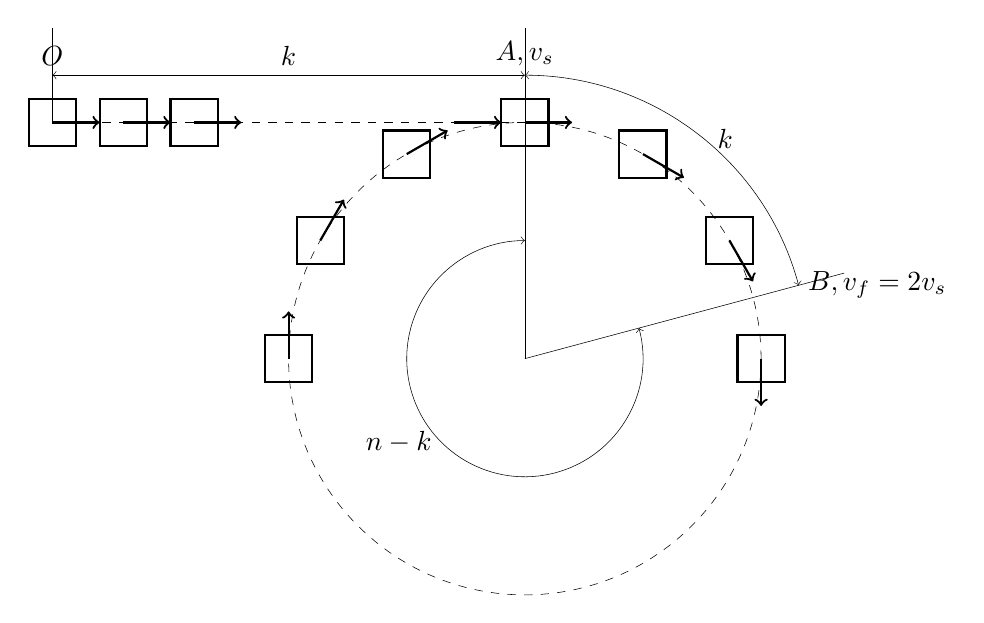
\begin{tikzpicture}[scale=3]
  % trace
  \draw[dashed, very thin] (-2cm, 1cm) -- (0, 1cm);
  \draw[dashed, very thin] (0,0) circle [radius=1cm];

  % label line
  \draw[very thin] (0, 0) -- (0, 1.4cm);
  \draw[very thin] (0, 0) -- (15:1.4cm);
  \draw[very thin] (-2cm, 1cm) -- +(0, 0.4cm);

  % label and arrows
  \draw[very thin, <->] (-2cm, 1.2cm) node[above]{$O$} -- (-1cm, 1.2cm) node[above]{$k$} -- (0, 1.2cm) node[above]{$A, v_s$};
  \draw[very thin, <->] (0, 1.2cm) arc [start angle = 90, end angle = 15, radius=1.2cm] node[right]{$B, v_f = 2v_s$};
  \draw (45:1.2cm) node[above]{$k$};
  \draw[very thin, <->] (15:0.5cm) arc [start angle = 15, end angle = -270, radius=0.5cm];
  \draw (-135:0.5cm) node[left]{$n-k$};

  % leading nodes
  \foreach \x in {-2, -1.7, ..., -1.4} {
    \draw[thick] (\x cm, 1cm) +(-0.1, -0.1) rectangle ++(0.1, 0.1);
    \draw[thick, ->] (\x cm, 1cm) -- +(0.2, 0);
  }

  % cricular starting points
  \draw[thick, ->] (-0.3cm, 1cm) -- (-0.1cm, 1cm);

  % circular nodes
  \foreach \deg/\rot in {90/0, 60/-30, 30/-60, 0/-90, 180/90, 150/60, 120/30} {
    \draw[thick] (\deg : 1cm) +(-0.1, -0.1) rectangle ++(0.1, 0.1);
    \draw[thick, ->] (\deg : 1cm) -- +(\rot : 0.2);
  }
\end{tikzpicture}
\caption{Two pointers solution.}
\label{fig:circular-catching}
\end{figure}

Let's consider the case that $k \geq n$. When the slower pointer arrives at $A$, The faster
one points to $B$ which is $k \bmod n$ nodes ahead. The faster one will catch
the slower one by eliminating their distance of $n - (k \bmod n)$ nodes.

\begin{equation}
\begin{array}{rl}
T & = \displaystyle \frac{n - (k \bmod n)}{v_f - v_s}\\
  & = \displaystyle \frac{n - (k \bmod n)}{v_s}
\end{array}
\end{equation}

When they meet again, the slower pointer has passed $v_sT = n - (k \bmod n)$ nodes.
The meet point is $k \bmod n$ nodes before $A$. We have the same result, that if
we reset the faster pointer to the head of the linked-list, and make the two pointers
advance one node per step, they will meet at $A$.

The following algorithm locates the node where the loop starts.

\begin{algorithmic}[1]
\Function{Find-Loop}{$L$}
  \State $p \gets q \gets L$
  \While{$p \neq $ NIL $\land q \neq$ NIL}
    \State $p \gets$ \Call{Next}{$p$}
    \State $q \gets$ \Call{Next}{$q$}
    \If{$q=$ NIL}
      \State break
    \EndIf
    \State $q \gets$ \Call{Next}{$q$}
    \If{$p = q$}
      \State $q \gets L$
      \While{$p \neq q$}
        \State $p \gets$ \Call{Next}{$p$}
        \State $q \gets$ \Call{Next}{$q$}
      \EndWhile
      \State \Return $p$ \Comment{Or return $q$}
    \EndIf
  \EndWhile
  \State \Return NIL \Comment{No loop}
\EndFunction
\end{algorithmic}

The following ANSI C example program implements this solution.

\lstset{language=C}
\begin{lstlisting}
struct Node* find_loop(struct Node* h) {
    struct Node *a, *b;
    a = b = h;
    while (a && b) {
        a = a->next;
        b = b->next;
        if (!b) break;
        b = b->next;
        if (a == b) {
            for (b = h; b != a; a = a->next, b = b->next);
            return a;
        }
    }
    return NULL; /*no loop*/
}
\end{lstlisting}

This solution is linear. The slower pointer exactly visits all nodes ($n + k$) when there is a circle.

\section*{Brent's algorithm}
Richard P. Brent described another linear time solution. If there is a circle with
circumference of $n$, start from any point in the circle, a runner will eventually
pass the same point after $n$ steps.

As illustrated in figure \ref{fig:circular-catching}, start from any node behand the
$k$-th one should be OK. The problem is how to reach such a point. Brent's idea
is to find the smallest number $m = 2^i$, that $m > k$ and $m > n$ for $i = 0, 1, 2, ...$.
We expect that after advancing some nodes, if we enter the circle, we can calculate
$n$ out within $m$ steps.

\begin{algorithmic}[1]
\Function{Cycle-Length}{$L$}
  \State $p \gets q \gets L$
  \State $n \gets 0$
  \State $m \gets 1$
  \Repeat
    \If{n = m}
      \State $p \gets q$
      \State $m \gets 2m$
      \State $n \gets 0$
    \EndIf
    \If{$b = $ NIL}
      \State break
    \EndIf
    \State $q \gets$ \Call{Next}{$q$}
    \State $n \gets n + 1$
  \Until{$p =$ NIL $\lor q =$ NIL $\lor p = q$}
  \If{$p =$ NIL $\lor q=$ NIL}
     \State $n \gets 0$
  \EndIf
  \State \Return $n$
\EndFunction
\end{algorithmic}


The complete ANSI C example program with test is distributed with this article.

\section*{Further reading}
Circular list is a special case of general Cycle detection problem \cite{wiki-cycle-detection}.
For any function $f$ maps finite set $S$ to itself with any initial value $x_0$, the sequence of the
iteration:

\[
x_0, x_1 = f(x_0), x_2 = f(x_1), ...
\]

must repeat. between some $i \neq j$, $x_i = x_j$. The cycle detection problem is to find $i$ and $j$ for
given $f$ and $x_0$. The method described here is invented by Robert W. Floyd in later 1960s, as known
as the `tortoise and the hare' algorithm. Brent's algorithm is described in
\cite{wiki-cycle-detection}.

\begin{thebibliography}{99}

\bibitem{Stepanov09}
Alexander Stepanov, Paul McJones. ``Elements of Programming''. Section 2.3, Chapter 2. Addison-Vesley Professional; (2009)

\bibitem{TAOCP2}
Donald E. Knuth. ``The Art of Computer Programming, Volume 2: Seminumerical Algorithms (3rd Edition)''. Addison-Wesley Professional; (1997)

\bibitem{wiki-cycle-detection}
Cycle dection. Wikipedia. http://en.wikipedia.org/wiki/Cycle\_detection

\end{thebibliography}

\end{document}
